%************************************************
\chapter{Flexible Event Subscription in BPMN}\label{ch:flexibleeventsubscription}
%************************************************

Given the requirements \textit{R1-R3}\,(see~\autoref{ch:requirements},\,p.\,\pageref{ch:requirements}) and the shortcomings \textit{S1-S3}\,(see~\autoref{ch:ass:discussion},\,p.\,\pageref{ch:ass:discussion}) identified in the previous chapters, this section presents an extension to the BPMN event handling model that allows the flexible use of event subscription mechanisms in business processes.

At first, \ref{ch:bpmnx} describes an extension to the \acf{BPMN}, which aims at providing the Process~Designer with a convenient solution for modeling events that must be obtained through the publish-subscribe interaction pattern.
Afterwards, \autoref{ch:automaticsubscription} clarifies the changes necessary to the event handling platform and the process engine to implement the implicit subscription management required by the BPMN extension.


\missingfigure{The concept for flexible event subscription involves three modules: A BPMN extension, enhanced process engine behavior and buffered event handling.}
\label{fig:concept-modules}

\section{BPMN Extension}\label{ch:bpmnx}

% maybe cite braun2015behind

The extensibility mechanism of the \ac{BPMN} allows to extend standard process elements with additional attributes, while maintaining conformity with the BPMN core~\cite[p.\,44]{bpmnspec}.
Extensions are specified through an external definitions file and can be included into a BPMN process model by reference.

\todo[inline]{write a little more about bpmn extensibility, then section structure}

- utilizing this mechanism, we propose a BPMN extension for flexible event subscription

-> refer to as befes? or just "the extension"
- structure of this section: overview (initial understanding of the extended notation and the semantics), usage documentation(, detailed execution semantics?)

\subsection{Overview}
This section introduces a novel BPMN extension for incorporating event subscription semantics in business process models.
The extension develops around the addition of subscription-related attributes to the BPMN \textit{Message} type. Based on the additional information, subscription and un-subscription for message events is handled automatically by an especially adapted process engine.
The added attributes are \textit{EventQuery}, \textit{SubscriptionTime} and \textit{BufferPolicies}:
\textit{EventQuery} contains an arbitrary query string; \textit{SubscriptionTime} defines when the subscription should happen; \textit{BufferPolicies} is a complex type which influences the behavior of the related event buffers.
Only \textit{EventQuery} is a mandatory parameter, all others will fall back to default values if not provided.
An overview of all possible fields, values and their defaults is provided in \autoref{tab:bpmn-extension}.

% variables in the event query

The presented extension is to be used in connection with intermediate catch events, boundary events and receive tasks through their direct or indirect association with the message element.
Additionally, the \textit{Event Subscription Task}, an extension of the \textit{Task} is introduced. It adds a single additional attribute \textit{messageId} to \textit{Task} and can thereby be used to manually trigger the subscription for the associated message element as part of the execution flow of a process.
%- for the others, the subscription and unsub from the event source is managed implicitly by the underlying infrastructure
By the use of the \textit{subscriptionTime} variable, the event subscription can be issued before the process flow reaches the event element and listens for the message. %bpmn event element is listening.
Any messages that arrive before the event element is active are temporarily stored and will be delivered to the catch event or receive task once it is active.
These storages as referred to as \textit{Event~Buffers}. By default, they store the latest message they receive, though the behavior can be adjusted using the \textit{BufferPolicies}.
The extension elements are illustrated through a UML-representation in \autoref{}, the formal XSD-Schema is available in the appendix, \autoref{lst:xsd-flexsub}.\todo[inline]{fix ref}

%- it is required that the infrastructure is prepared to execute extended processes accordingly, ref chapter
% though, theoretically, every message can be extended with the attributes, the subscription is only managed for the elements...

\missingfigure{UML-Diagram of BPMN extension: task>expl subscr task; message > messageeventdef > interm catch event; message > receive task}


\begin{table}
	\myfloatalign
	\begin{tabularx}{\textwidth}{p{0.3\linewidth} p{0.515\linewidth} c}
		\toprule
		\tableheadline{Attribute Name} & \tableheadline{Value Options (\underline{default})} & \tableheadline{Req.} \\ 
		\midrule
		EventQuery & any query string & y \\
		SubscriptionTime & process-deployment,\newline process-instantiation,\newline manual, \underline{element reached} & n \\
		BufferPolicies & Complex Type (see below) & n \\
		
		\midrule
		\tableheadline{bufferPolicies}  \\
		\midrule
		
		LifespanPolicy & string in ISO time-span format OR '\underline{infinite}' & n \\
		ConsumptionPolicy & \underline{reuse}, bounded-reuse(n), consume & n \\
		SizePolicy & positive integer, \underline{1}, 0 means infinite & n \\
		OrderPolicy & \underline{FIFO}, LIFO & n \\
		
		\bottomrule
	\end{tabularx}
	\caption[]{Available attributes of <subscriptionDefinition> in the BPMN extension for flexible event subscription}  \label{tab:bpmn-extension}
\end{table}

\subsection{Documentation}

> why everything is added to the message element


Semantically, the \textit{Message} type is most suited to be extended with subscription information.

% receiveTask.messageRef; boundaryEvent.catchEvent.(message)eventDefinition.messageRef; intermediateCatchEvent.catchEvent.(message)eventDefinition.messageRef
Each of the three elements references a BPMN \textit{Message}, the common denominator for communication within and across business processes.

\todo[inline]{mention that others have extended the events instead, but this proposal goes another way}

\todo[inline]{explain that the Message is a common element in BPMN models. It is the main generic type used for communication, collaboration.
	The proposed extension to the Message type is only to be used by Message Receive situations in Intermediate Catch Event, the Boundary Catch Event and the Receive Task.}

By specification, \textit{tMessage} comprises an attribute \textit{name}, the name of the message, and \textit{itemRef}, the reference to a BPMN \textit{ItemDefinition}. Additionally, it inherits all attributes from the BPMN \textit{RootElement}.
In the following, the required additional attributes will be explained one after the other. A complete list is available in \autoref{tab:bpmn-extension}. The goal is to retain a stand-alone model that contains all information necessary to execute the subscription to the event source.

- information is added to <subscriptionDefinition>

%\subsubsection{Introducing Event Buffers}
%Any event message that occurs before reaching the event element but after the time of subscription will be kept in a buffer by the system.
%In its simplest version, the buffer is of length 1, that means it stores exactly one message received from a CEP platform. It always stores the latest message. When a newer message arrives, the old one is replaced in the buffer.
%\autoref{ch:bpmnx:bufferpolicies} introduces a set of advanced buffer policies to adapt this behavior further.
%\todo[inline]{By default, there is no interference between the buffers of different messages, process instances or processes. Each buffer instance will contain the latest information as if it was the only buffer in the system. Performance improvements to avoid duplicate buffer content will be managed by the system without explicit action by the user. Section ... later introduces a shared, more complex usage scenario of the event buffers.}

\subsubsection*{Adding basic subscription information}\label{ch:bpmnx:basic}

For a subscribe operation, we consider the event~query, the platform address and optionally authorization information of the CEP~platform.
This extension assumes that only one event engine is in use, so that access information can be configured in a central configuration store for the current process execution environment and not redundantly for each message.
The event query instead needs to be specified for every message and is added to the model as an extension attribute \textit{eventQuery} of type \textit{string}, which should contain the full query as interpretable by the CEP platform.

A similar approach has been taken by X and Y, who aim at enriching BPMN models with subscription information without considering the time of subscription specifically.
\todo[inline]{Find this source; explain what they do (different)}

Given this first fundamental part of the BPMN extension, it is possible to execute the subscription, but the time of subscription cannot be influenced.

\subsubsection*{The time of event subscription modeled in BPMN}\label{ch:bpmnx:subscriptiontimes}

This section specifically addresses the requirement \textit{R1.1}, aiming to provide a flexible event subscription time to be selected for each BPMN message when designing an event-driven process.
Two different means are to be offered to support all subscription times demanded by \textit{R1.1}: Firstly, the subscription can happen in the background. Alternatively, the subscription can be modeled explicitly as a flow-element in the process.
It is a task of the process design phase, to elaborate the correct time of subscription necessary for the use case.

The subscription will be executed automatically by the system based on the information given in the BPMN model. Further information on the exact execution flow is provided in chapter~XY.

\todo[inline]{Time of un-subscription also must be clarified in bpmnx}


\paragraph{Subscription time as part of the BPMN Message element\newline}
To provide the Process Designer with a simple but powerful tool to influence the time of event subscription, a field \textit{subscriptionTime} is added the BPMN message element. 
The field can take one of the following values: \textit{process-deployment}, \textit{process-instantiation}, \textit{manual}, \textit{element-reached}. The last option is the default option, intepreting the standard BPMN semantics.
Note that a \textit{subscriptionTime} set to \textit{element-reached} will remain without effect if an explicit subscription task for the same event was executed before the event is reached.

\todo[inline]{For each of the options: Define exactly (according to BPMN spec or standard literature), when in the flow the subscription is executed.}

In motivating Example~1.1, it is necessary to issue the subscription to the Eurotunnel event as early as possible to make sure that data is available and the process execution is not delayed.
Using the BPMN extension, the use case can be implemented by defining the event query and the subscription time in the BPMN model. \todo[inline]{show what that would look like in the example. Maybe some XML?}

\paragraph{The event subscription task\newline}
As an alternative to specifying the subscription time using the extension field \textit{subscriptionTime}, an extension to the BPMN \textit{Task} type is proposed. \todo[inline]{it follows the ideas presented in ... but through referencing the message element}
Other than \cite{mandal:2017} 



\missingfigure{Example 2 using an explicit subscription task}

The extended task is used to execute the subscription explicitly as part of the process flow.
A field \textit{messageId} is added to the service task to establish a reference between the activity and the message definition.
As introduced in section~\autoref{ch:bpmnx:basic}, the extended BPMN Message definition contains the information necessary to issue the subscription to an event source.
Once the Explicit Subscription Task is activated, the subscription for the referenced message is issued. 

Modeling the event subscription in an explicit task can be necessary when the subscription depends on the result of another activity. In that case, the subscription cannot be issued on process instantiation, because the necessary information is not yet available. Instead, an early subscription can be implemented using the extended service task.
Apart from this particular use case, the explicit subscription task enables the Process Designer to place the subscription flexibly in the process flow and give her full control over the time of subscription.

\todo[inline]{As an improvement to the options for subscription time, there could be an option "ASAP", so that the process engine issues the subscription automatically as soon as the required process data becomes available}

If both tools, the extension field \textit{subscriptionTime} and the explicit subscription task, are used for a single BPMN message, the earlier subscription of the two will be executed, the second subscription will have no effect.
That means for example if the \textit{subscriptionTime} is set to \textit{event reached} and an explicit subscription task is inserted before the event element, then the subscription will be executed at the time the explicit subscription task is active.
If \textit{subscriptionTime} is set to \textit{Process Deployment}, then the subscription will happen at that time and the explicit subscription task will remain without effect.
In case neither of the two is used, the system falls back to the BPMN default and executes the subscription when the event element is reached.

\subsubsection{Using Process Variables in Event Queries}

% also see bpmn2 spec 10.3 pp. 233ff.

As shown in example~1.2, it can be the case that the current values of process data must be dynamically used in an event query. \todo[inline]{missingref}
Therefore, the name of the dataObject should be part of the event query. At the time of subscription, the mentioned variable is dynamically replaced by its current value.
The exact notation for including process variables in event queries may vary depending on the employed query language so that it does not interfere with any existing notation schemes.
For the use with the Esper EPL, the following is suggested: The exact name of the variable has to be surrounded by curly brackets and preceded by a \textit{\#} character: \textit{\#\{VARIABLENAME\}}.
This notation is inspired by the usage of substitution parameters in SQL queries that are embedded in Esper EPL. They take a similar form, though using a \$ sign\footnote{see~\textit{5.13.1. Joining SQL Query Results}, \url{http://www.espertech.com/esper/release-5.3.0/esper-reference/html/epl_clauses.html}, accessed 2017-08-13}.

\todo[inline]{brief recap of the example and show query using the variable. considering the value is stored in the dataObject ".."}
\textit{SELECT lat, lng from GPSUPDATE where truckid = \#\{truckid\} }.

The use of dynamic process variable values introduces an additional complexity: Depending on the time of event subscription, the value of the process variable might not yet be available.
\todo[inline]{only if subscriptionTime not 'on depl'}
\todo[inline]{What does this mean for the process designer? A model that can take a state in that a subscription shall be issued, though the data is unavailable, is invalid. When will an error occur? }


\subsubsection{Advanced Buffer Parameters}\label{ch:bpmnx:bufferpolicies}

\paragraph{Lifespan of buffered events\newline}

The \textit{LifespanPolicy} allows to specify after which timespan elements in the buffer should be deleted. Timespans are defined using the ISO8601 notation for time intervals\footnote{see \textit{Date and time format - ISO 8601}, \url{https://www.iso.org/iso-8601-date-and-time-format.html}, accessed 2017-08-13}. 
The default value is \textit{infinite}.

\todo[inline]{überleitung zu example}
Example~1.1 is implemented by setting the \textit{subscriptionTime} to \textit{process-deployment}, which means that there can be an infinite time difference between the action of subscribing to the event source and the reaching of the event element in one of the instances. \todo[inline]{ref example}
In case events are not published in a longer time, for example due to technical fault at the event producer, the buffer will contain older events that might not be relevant anymore.
Using the \textit{LifespanPolicy}, the process designer can express, that events should be deleted from the buffer after a certain period of time and thus avoid outdated information. The buffer is maintained automatically by the system.
That of course comes at the price that the process has to remain in waiting state until a new event message arrives.

\paragraph{Consumption Behavior\newline}

So far, the event buffers can be used isolated from each other. There is no interference between buffer instances and events are not removed from the buffer after retrieval.
While for most use-cases this behavior is sufficient, more detailed control over the buffer can be desirable when a given message is accessed multiple times. More precisely, if an event element is activated multiple times or multiple elements reference the same \textit{Message} element, then the consumption behavior must be clear.
Not always is it wanted, that events remain in the buffer after retrieval.
An additional parameter \textit{ConsumptionPolicy} is introduced which can take the values \textit{consume}, \textit{reuse}(default) and \textit{bounded reuse(n)}.
While \textit{reuse} denotes the behavior that is already known, \textit{bounded reuse(n)} will allow an element to be retrieved exactly \textit{n} times. \textit{n} has to be replaced by an integer value greater 0.
The option \textit{Consume} will remove an element from the buffer immediately after it has been retrieved for the first time, it is therefor equivalent to \textit{Bounded Reuse(1)}.

\todo[inline]{can still be clearer}


\begin{figure}[]
	\myfloatalign
	{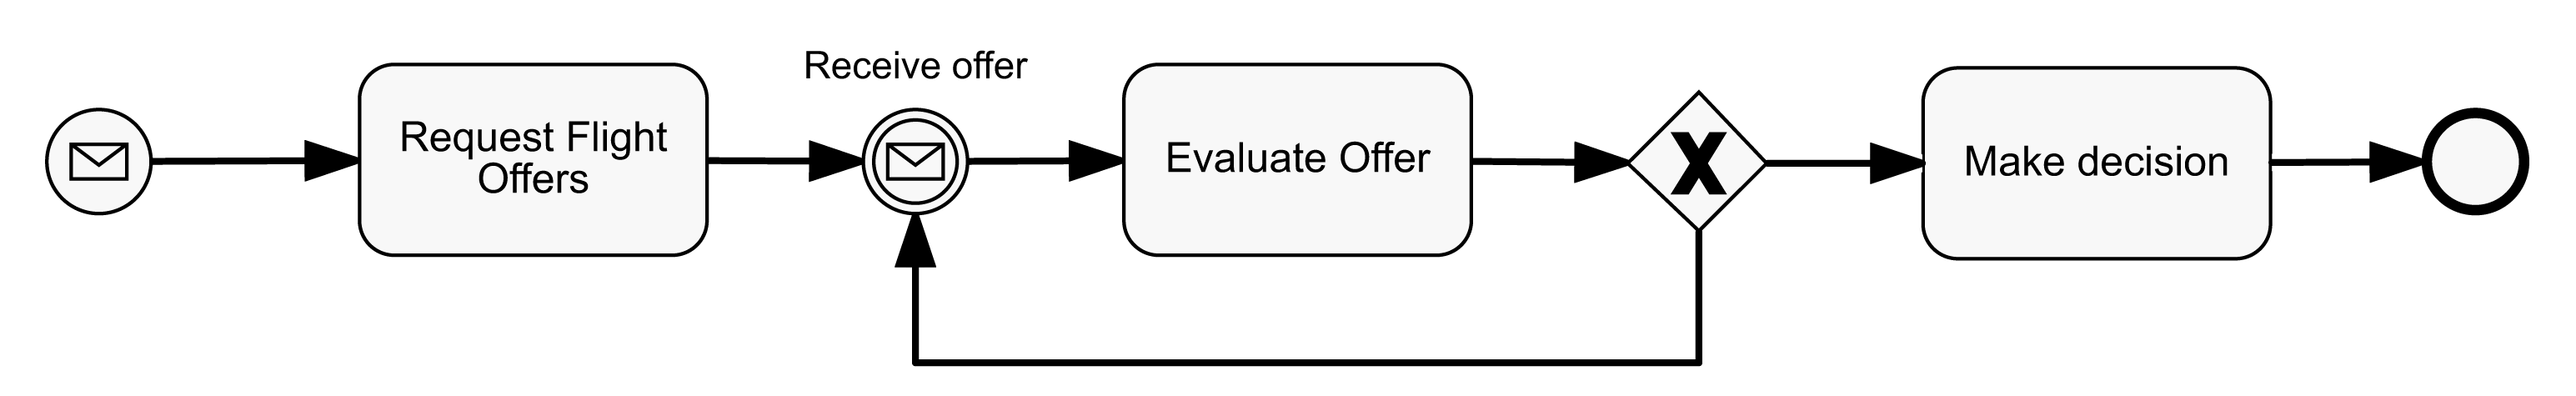
\includegraphics[width=1\linewidth]{chapters/concept/bpmnx/FlightBooking.png}}
	\caption{Flight Booking process using a consuming buffer}\label{fig:example-flightbooking}
\end{figure}

\todo[inline]{write about the examples}

- given the option to consume from the buffer, it will now make a difference if the same buffer is accessed multiple times.
- there are two scenarios to access the same buffer: (1) multiple times in the same instance, (2) multiple times because of parallel instances, (3) multiple times because of a shared buffer across processes
- before proceding, we need to be clear about the buffer scope: it depends on the time of subscription. (1) after instantiation: buffer only instance-wide; (2) on pr depl: buffer reused across all instances; (3) buffer reused across all processes if messageId and query are the same.

\begin{figure}[]
	\myfloatalign
	{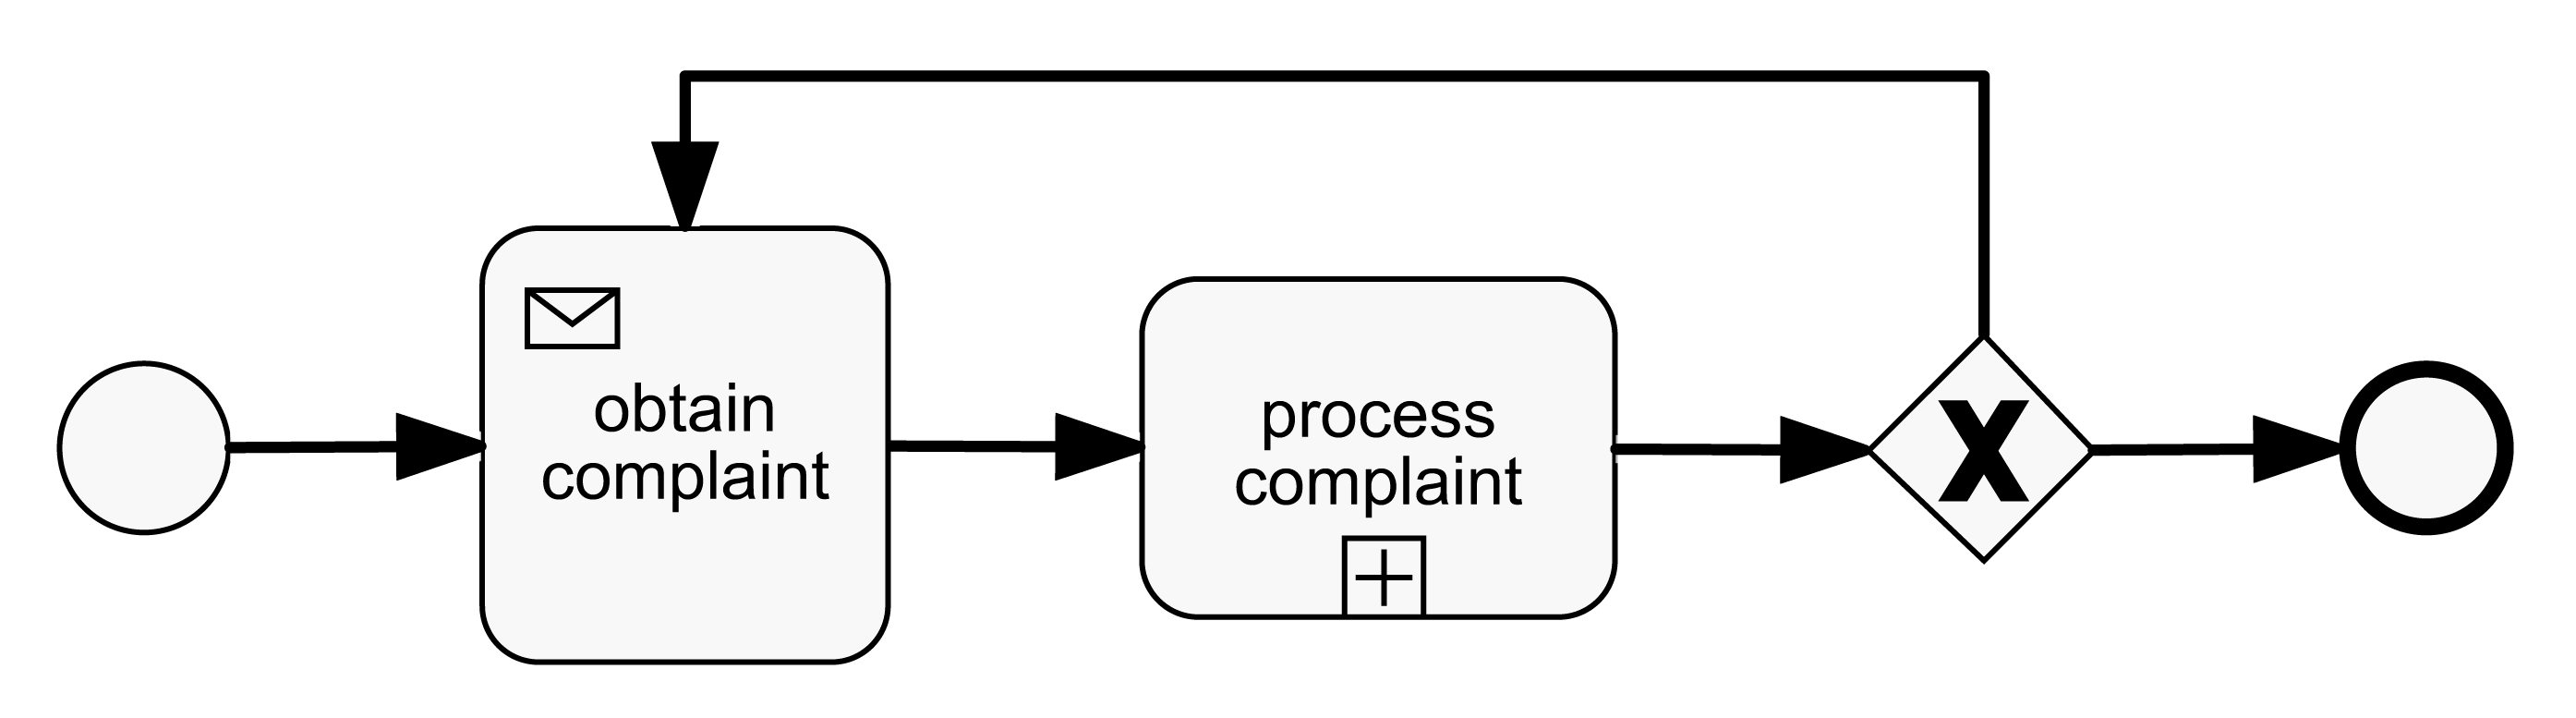
\includegraphics[width=1\linewidth]{chapters/concept/bpmnx/ComplaintProcessing.png}}
	\caption{Shared consuming buffer in Complaints Handling}\label{fig:example-complaints}
\end{figure}

\paragraph{Buffer Size and Order Policy\newline}

- two additional buffer policies: \textit{SizePolicy}, \textit{OrderPolicy}, default values
\todo[inline]{write text for given keypoints}

- what if messages are defined in different ways? => I want to reuse the buffer between processes, but the message definition (especially cep query) are not the same. how will the system behave?

\paragraph{Interplay of Event Queries and Buffers}

// even with the simplest settings

Modern event query languages are feature-rich and offer a large set of expressions to filter events from incoming streams. \todo[inline]{ref background}
The introduced basic event buffer can be used in connection with any desired event query and will store the latest output of that query.
These two features together suffice to implement even more complex use-cases: Query windows of length \textit{n} can be used to keep multiple events in the buffer, filter expressions allow to keep a subset of all events based on their attribute values, multiple streams can be joined together.
As soon as the process flow reaches an event element, the latest CEP message is retrieved from the buffer. It is not consumed, that means a second event element that references the same BPMN Message will reuse the information from the buffer.
If no information is available in the buffer, the flow element will remain in the waiting state until a message is received. Then, the process flow proceeds as usual.

\subsection{Execution Semantics}

%************************************************
\section{Automatic Subscription Handling}\label{ch:automaticsubscription}
%************************************************

After defining the notation and functionality provided to the user through the BPMN extension for flexible event subscription, this chapter describes the changes necessary to the software infrastructure to implement the execution semantics.
The concept requires that all subscription operations and event handling is executed by the system itself, solely based on the extended BPMN model.
Changes are necessary to both, the event processing module and the process engine. This chapter attempts to keep the change descriptions general so they can be applied to any common process engine and event processing platform.
The first section describes the necessary extension to the event processing so that a delayed delivery of events is supported.
The following \autoref{ch:extendedprocessengine} specifies the changes necessary to the behavior of the process engine as the connecting element between the BPMN model and the event processing platform.


\subsection{Buffered Event Processing}\label{ch:bufferedcep}
When reduced to the basics, a standard event processing platform works as follows: The user subscribes to events providing an event query and a notification-path. The platform responds with a unique identifier for that subscription.
Whenever an event occurs that matches the provided query, the platform issues a notification to the notification-path. Subscriptions can be deleted through their unique identifier.
These two operations, \textit{subscribe} and \textit{unsubscribe}, make the fundamental \acs{API} of a CEP platform~(see \autoref{ch:bg:cep}).

\paragraph{An API for buffered event processing}
The novel BPMN extension for flexible event subscription allows to issue a subscription to an event source well before the events ought to be delivered to the process instance. The introduction of an event buffer as a separate entity between the notification-recipients and the event query makes an adaptation of the API necessary.
In the following, we propose an API for buffered event processing which provides the functionality necessary to implement the execution semantics specified in the BPMN extension. Note that the proposal is not restricted to a certain kind of technology or protocol to implement the API.

Firstly, the \textit{subscribe} operation has to be available in two steps:

\begin{aenumerate}
	\item \textit{registerQuery(queryString[, bufferPolicies]): queryId}\newline
	The call registers an event query in the CEP platform and instantiates a buffer. Matching events will be held in the buffer according to the specified  policies. It returns a unique identifier to that new query registration and hence for the connected buffer. That identifier must be used to modify the query later.
	
	\textit{bufferPolicies} is an optional parameter which is provided as an object with four possible fields: \textit{LifetimePolicy}, \textit{ConsumptionPolicy}, \textit{SizePolicy}, \textit{OrderPolicy}. Refer to \autoref{ch:bpmnx:bufferpolicies} for a detailed specification of the semantics and possible values of the parameters. If \textit{bufferPolicies} is not or only partly specified, the system should fall back to the denoted default values.
	
	\item \textit{subscribe(queryId, notificationPath): subscriptionId}\newline
	Initiates the delivery of notifications for a given queryId to a notification recipient.
	The recipient is specified through the \textit{notificationPath}, the full address of the entity that is supposed to receive the message.
	Notifications are delivered asynchronously as soon as they are available. If the buffer is not empty, a message will be sent right after the \textit{requestEvents} call.
	A similar operation, \textit{addNotificationRecipient}, is available in existing CEP platforms. It adds a notification recipient to a query that is already registered in the platform. The difference is in the delivery of the first buffered message: \textit{requestEvents} sends out the message from the buffer, \textit{addNotificationRecipient} will send out notifications only for future query output.
\end{aenumerate}\label{def:apiextension-subscribe}

\noindent A similar situation holds for the un-subscribe operation: Given flexible event subscription, the operation must comprise of two steps:

\begin{aenumerate}
	\setcounter{enumi}{2}
	\item \textit{unsubscribe(subscriptionId)}\newline
	Removes a notification-recipient for a given query-id. Note that the buffer and query instance remain intact, so that other recipients can still subscribe.
	\item \textit{removeQuery(queryId)}\newline
	Completely deletes the query and its buffer, so that no notifications are sent out any longer. 
\end{aenumerate}\label{def:apiextension-unsubscribe}

\noindent
All four methods must be available to execute a subscription before process deployment.
The query must be registered using \textit{registerQuery} before the process instance, and hence the notification-path, is available. For each process instance, a subscription can be issued individually using \textit{subscribe} and thereafter, the notification-recipient can be removed with \textit{unsubscribe}.
The query and its buffer will remain active even after any single instance has terminated. When the process gets un-deployed, the query can be deleted using \textit{removeQuery}.
%\autoref{ch:extendedprocessengine} describes the steps in detail.

\todo[inline]{show the steps with sample data from one of the examples}


\paragraph{Architectural options}

Three options are considered to implement the explained functionality~(\autoref{fig:buffered-event-handling-architecture}). 
(a) It can either be implemented by adopting the CEP platform itself, (b) by implementing a separate middleware between process engine and CEP platform, (c) or by implementing a buffering module as part of the process engine.
Which of the three options suits best has to be evaluated for the given use-case and existing infrastructure. In some cases it might not be possible to adapt the code of process engine or event processing platform, which leaves a separate middleware as the only choice.

\begin{figure}[]
	\myfloatalign
	{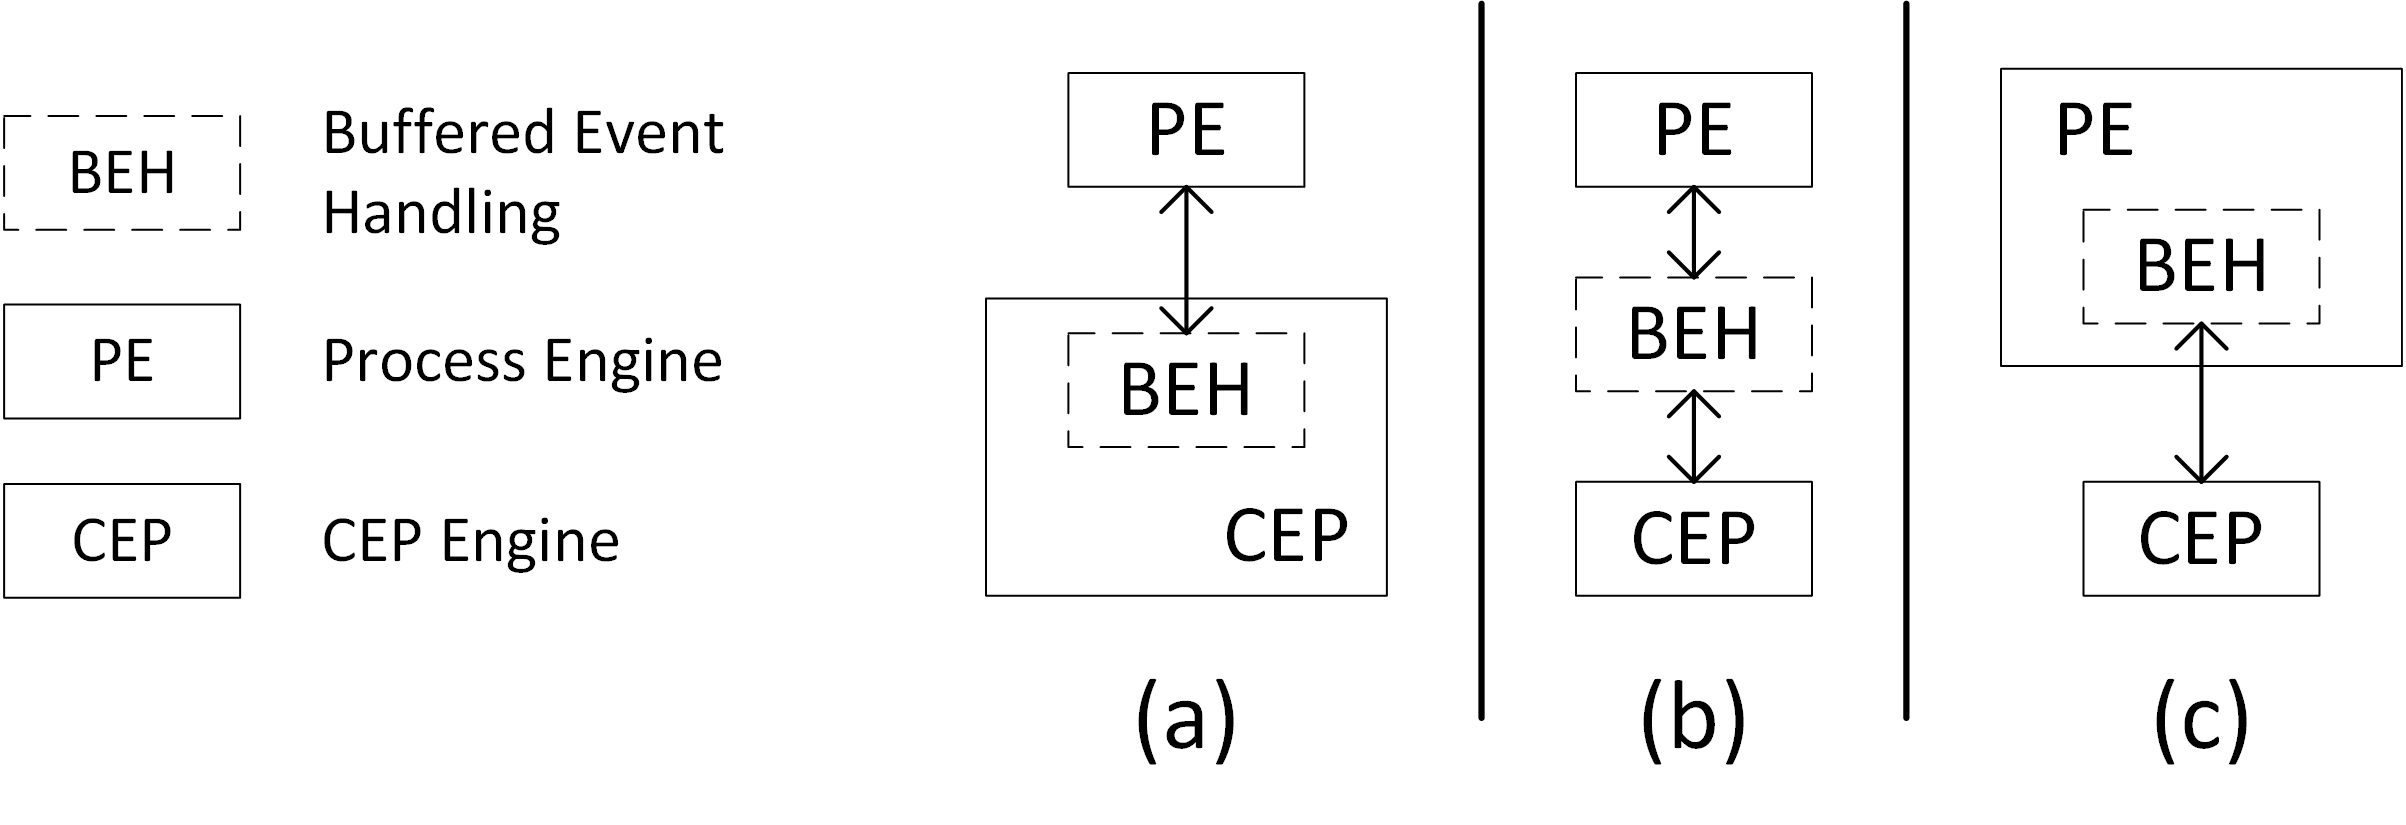
\includegraphics[width=0.8\linewidth]{chapters/concept/automaticsubscription/architecture-options.png}}
	\caption{Architectural options to implement the event buffers}
	\label{fig:buffered-event-handling-architecture}
\end{figure}

A reference implementation for an extended complex event processing platform is presented in \autoref{ch:implunicorn} at the example of the Esper-based CEP~platform \textit{Unicorn}. It also explains, why extending the event platform was the preferred choice in the given scenario.

\medskip \noindent
- given the extended api, it is now possible to implement early event subscription from the process engine
\todo[inline]{connector}


\subsection{Extended Process Engine Behavior}\label{ch:extendedprocessengine}
It is the task of the Business Process Engine to interpret and execute process models and connect to an event processing platform in event-driven setups.
From the three relevant parts, two have already been defined, the BPMN extension and the buffered event processing module.
Out of the box, a process engine like Camunda will ignore any proprietary BPMN extensions and the subscription to an event source must be especially implemented. An example for such an implementation is provided in \autoref{ass:model:buffered}.
One goal of this work is to automatize the handling of event subscriptions solely based on the information available through the extended BPMN model. Additional process elements should not be required.
This section will clarify, which operations need to be executed by the process engine to enable the automatic subscription handling.
\autoref{ch:implcamunda} demonstrates the implementation of automatic subscription handling at the example of Camunda.

\paragraph{Parsing additional information from the BPMN model}
It is required that the process engine is able to read the additional information from the BPMN extension~(see~\autoref{ch:bpmnx}) so that it is available during process deployment and execution.
This affects the BPMN message element, which can contain the additional attributes \textit{eventQuery}, \textit{subscriptionTime} and \textit{bufferPolicies}.
Secondly, the \textit{Event Subscription Task} has to be processed. It contains a reference to a Message entity within the same model element.
The process engine might have to be adopted to read all relevant data from the extended model.


\paragraph{Managing subscription and un-subscription}
As defined in the BPMN extension for flexible event subscription, the action of subscribing to an event source can happen at different times during process deployment and execution. The options and the implicit timing of subscription and un-subscription are specified in \autoref{ch:bpmnx:subscriptiontimes}.
The process engine must communicate with the process engine using the four calls \textit{registerQuery}, \textit{requestEvents}, \textit{unsubscribe} and \textit{deleteQuery}, that were presented in the previous chapter.
For each possible subscription time, the following briefly enumerates which operations must be executed when. 

\begin{description}
	\item[In every case:] 
		The return-value of \textit{registerQuery}, a unique identifier of that query, must be stored for the related BPMN \textit{Message}. The id is later necessary to execute the other three API methods.
		If the event query contains one or more variable values (see \autoref{ch:bpmnx:variables-in-queries}), all have to be replaced by their current values when \textit{registerQuery} is performed.
		When an event element is reached, a call to \textit{requestEvents} must be issued. When the execution of that event element is finished, call \textit{unsubscribe}.
	\item[Subscr. on process deployment:]
		When a process gets deployed, the process engine must check if subscription information is in the model. For every \textit{Message} element that is set as \textit{subscribe on pr. deployment}, a call to \textit{registerQuery} must be issued as part of the deployment process. A call to \textit{deleteQuery} is executed when the process gets un-deployed for the same messages.
	\item[Subscr. on process instantiation:] 
		When a process gets instantiated, \textit{registerQuery} must be executed for each \textit{Message} that is set to \textit{subscribe on pr. instantiation}. \textit{deleteQuery} can be called when the last reachable event element for a \textit{Message} has finished executing or no connected event can be reached anymore. The deletion happens at the latest when the process instance terminates.
	\item[Subscr. through explicit subscription task:]
		If the control flow reaches a subscription task, the process engine executes \textit{registerQuery} for the referenced \textit{Message}. The execution of \textit{deleteQuery} follows the same rules as in the preceding case.
	\item[Subscr. when the event element is reached:]
		Once the event element is reached, \textit{registerQuery} must be executed for any \textit{Message} that is not covered by one of the prior cases. \textit{deleteQuery} must be called when the event element is finished.
\end{description}
\todo[inline]{be more precise about the time the calls should be executed (if possible). "reached"? "completed"? use the right bpmn words}



\todo[inline]{write conclusions that repeat how each requirement has been fulfilled}

\section{Design Decicions}\label{ch:designdecisions}

The target functionality of the BPMN extension was clearly defined by the identified requirements.
To implement that functionality, there were a number of options to consider and design decisions to make.
This chapter provides background information on the decisions that have influenced the presented concept for flexible event subscription.

\todo[inline]{Talk about an alternative solution? Table of events for a certain event source. The buffer is already there for me to pick from when designing the process.}

\paragraph{The time of subscription is a question of process design}
-> process designer
- this is why the bpmn extension is presented first
- hide complexity from the designer

\paragraph{The actual buffer is mostly hidden from the user}

- Buffers are implicitly defined through the BPMN model
- keep the look and feel of the message catch event
- minimal changes to existing models, backwards compatibility

\paragraph{Avoid additional user interfaces}
- the user will only use the bpmn model
- we don't want any other element because of complexity
- the process should be self-contained, contain all necessary information for subscription and buffering.
-> single point of contact

\paragraph{Buffers are closely linked to process models}
Messages are only buffered as soon as they are explicitly required by a model
- we don't just buffer n messages because we might need them in the future. That would be a fuzzy, incalculable performance overhead.
- instead we keep as little as possible in the buffer

\paragraph{The BPMN Extension is based on the Message element}
- if I want to talk about related work that goes another way
- why are the policies a parameter of the message and not the catch event element?

\paragraph{reuse existing technology}
-> we assume that a cep is present and that basic features of event queries can be used
- if not present, then only very basic buffer functionality is available
- but we dont want to start designing another event processing layer with duplicated functionality
